\subsection{Experiment-1. 12.02.2020}\label{experiment-1.-12.02.2020}

The first attempt took place on 12.02.2020. 6 \Glspl{ue} took part ranging by \gls{android} version from 4 to 9.

\subsection{Weather conditions}

\begin{itemize}
	\tightlist
	\item
	no precipitation
	\item
	cloudy sky
	\item
	a thin layer of snow on the ground
	\item
	temperature of -1..+1$^\circ$
\end{itemize}

\subsection{Procedure}

All items of the experiment placed on carton boxes on the ground. Figure \ref{fig:cnc-position} shows a picture of \gls{command_n_center} position during the first trial of experiment.

\begin{figure}[H]
	\centering
	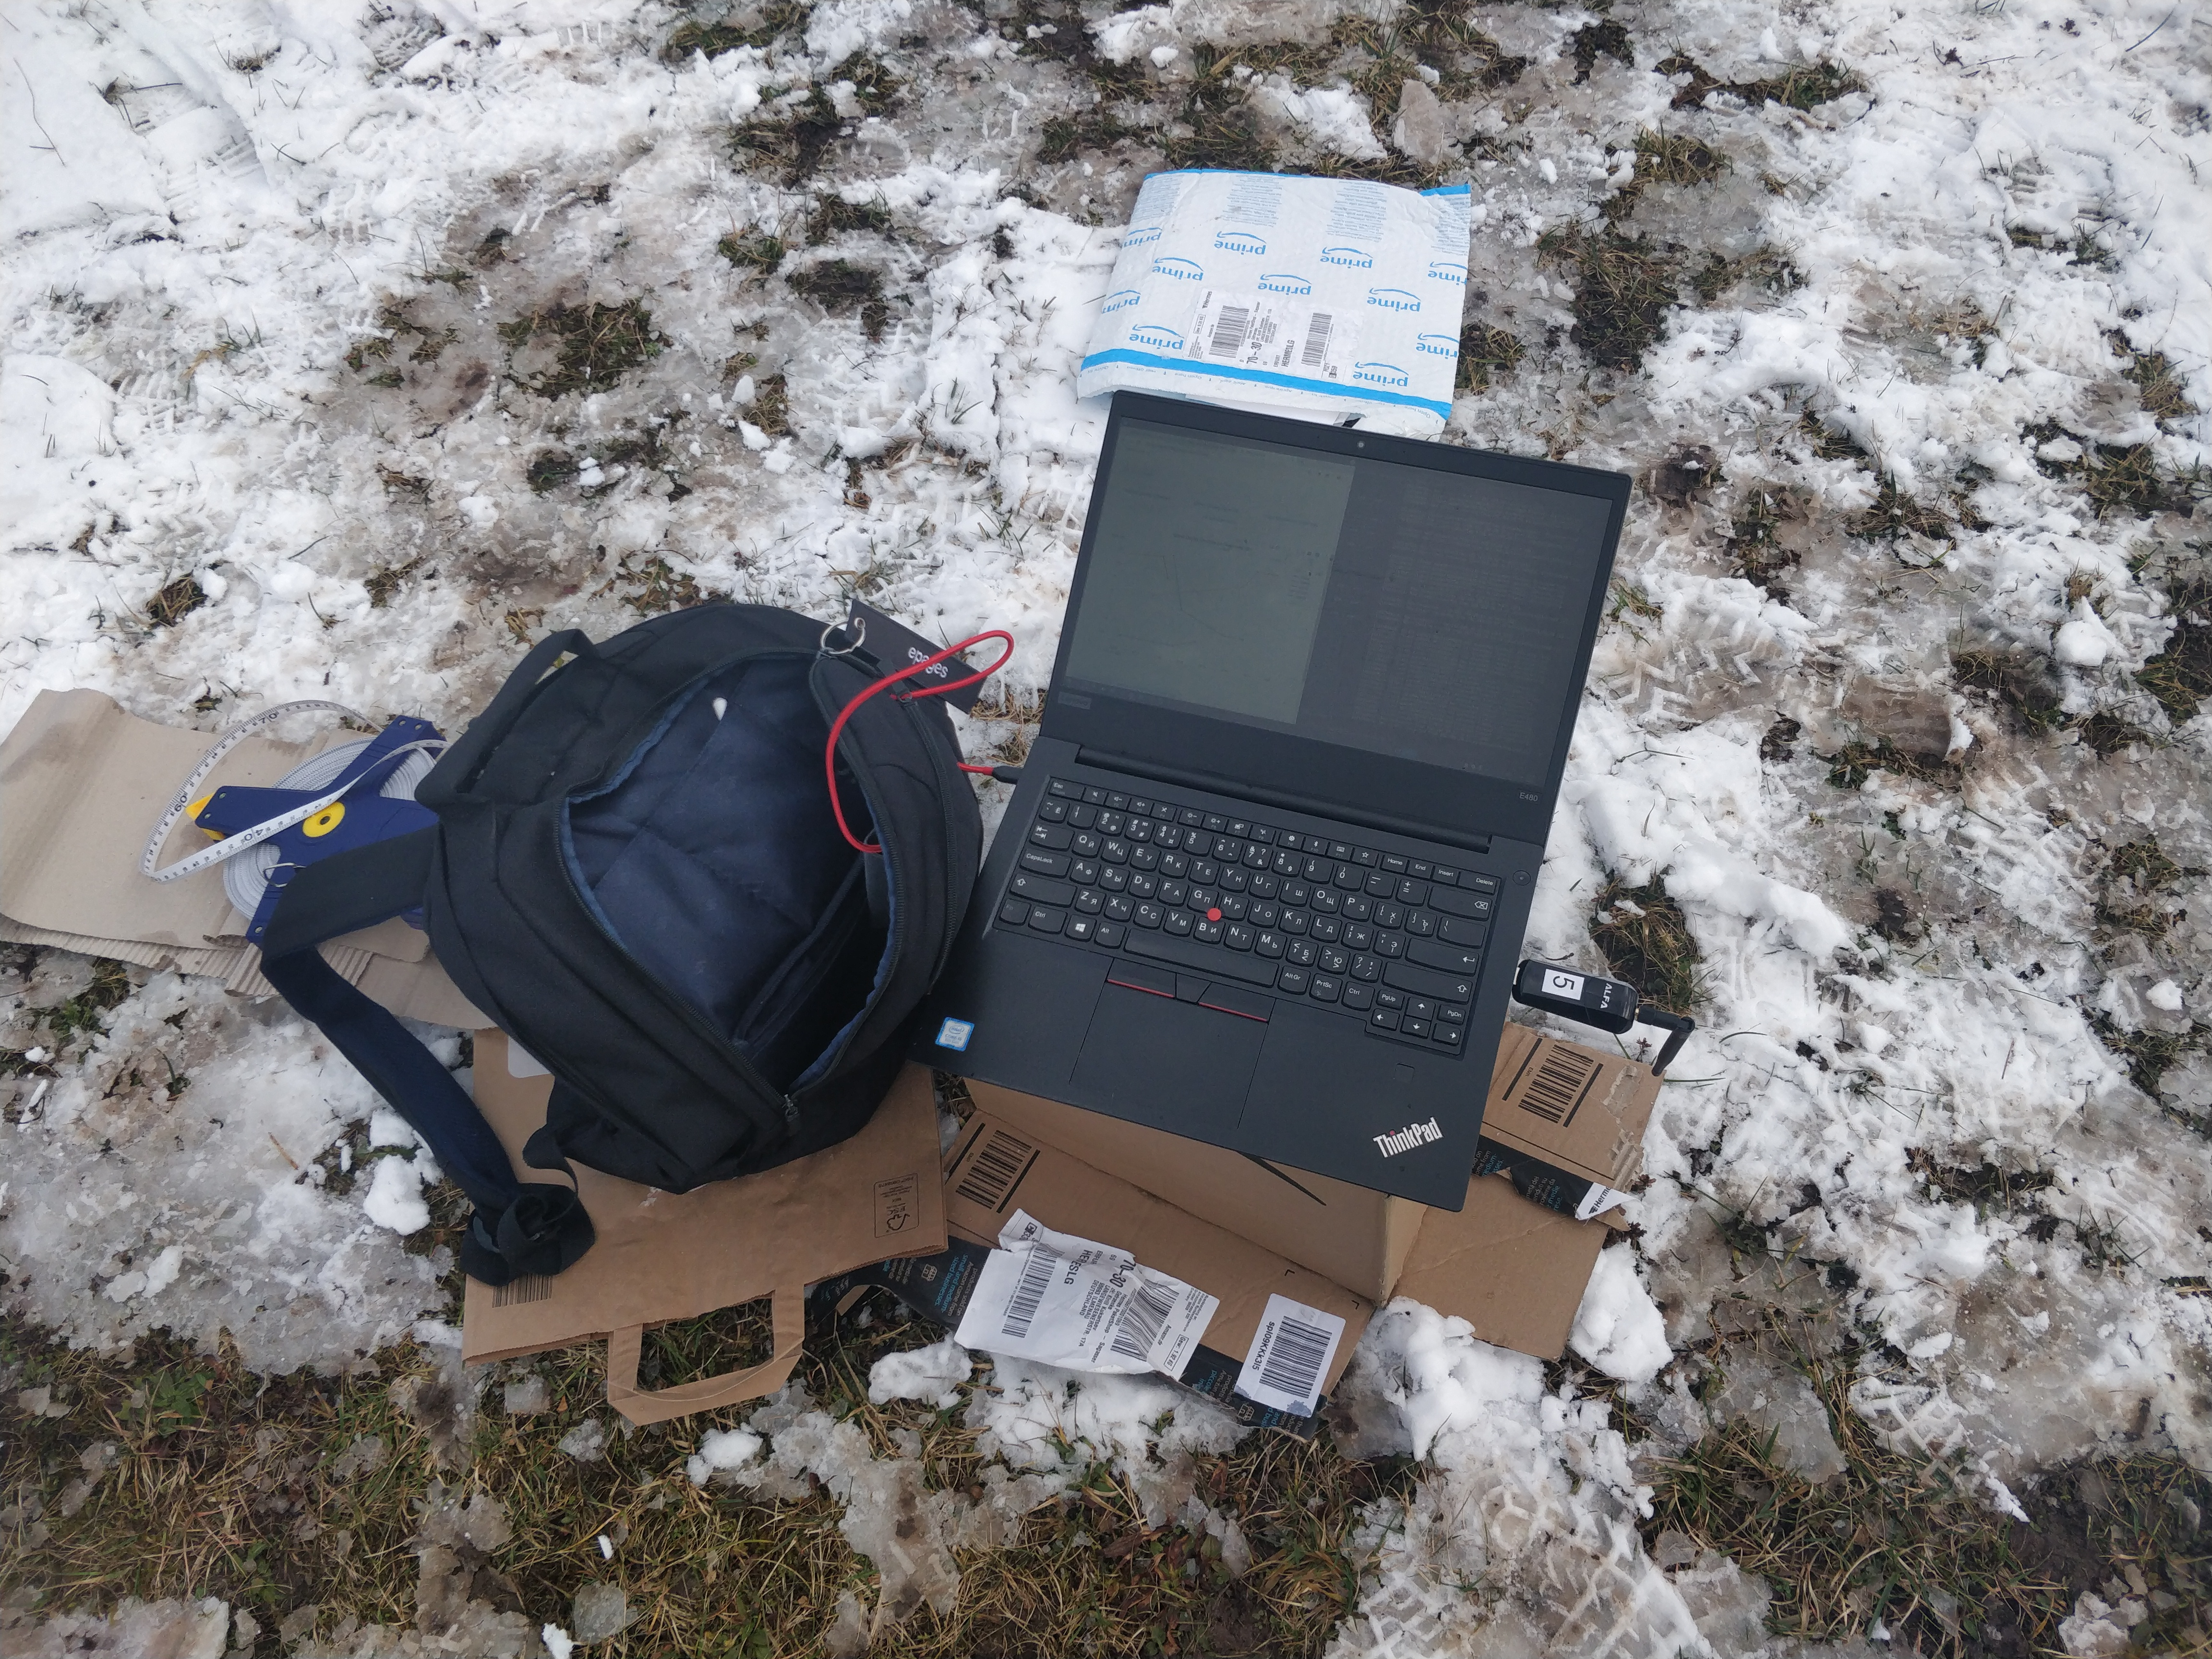
\includegraphics[width=0.6\linewidth,keepaspectratio]{images/experiment_1_cnc.jpg}
	\caption{Layout of \gls{command_n_center} server}
	\label{fig:cnc-position}
\end{figure}

\subsubsection{Case 1}

We started with \hyperref[sub-optimal-layout]{Sub-Optimal case}.

One \gls{ap} functioned correctly - one group of \glspl{ap} connection to one \gls{ap} was made successfully.
Here was a problem with the second group of \glspl{ap} - due to weather conditions we encountered \gls{wifi} module issues of \gls{ap} (the laptop freeze).

After some time of data collection, it was clear the second \gls{ap} was not sending data to \gls{command_n_center} at all, so we decided to locate devices according to \hyperref[near-optimal-layout]{Near-Optimal layout scheme}.

\subsubsection{Case 2}

During \hyperref[near-optimal-layout]{Near-Optimal layout case} we observed increase of \acrshort{rss} level -82 and -84 dBm for the left \gls{ap} to -76 and -80 dBm for the other. Link measurement messages from \glspl{ue} connected to the second \gls{ap} dropped by an unknown reason.

Moreover, \gls{gps_frontend} showed that some \glspl{ue} are close to each other (having approximately the same coordinate), whereas the other 2 were detected much further. It indicates that \glspl{gnss} position measurements are biased.

After, the second \gls{access_point} stopped working at some time. Restart and re-connection of \glspl{ue} did not help to obtain data.


\subsubsection{Case 3}

Because of the problems encountered in the previous case, we decided to stop the experiment and figure out possible solutions.

\subsection{Outcome}

The first trial showed:

\begin{itemize}
	\tightlist
	\item
	Further development and bug fixes of \gls{gps_tracker}  and  \gls{gps_android} required.
	\item
	Tests of placement algorithms can be performed, but due to problems with message sending, we could not prove that the suggested optimal positions would lead to better signal conditions.
\end{itemize}

As a result, we decided to:

\begin{itemize}
	\tightlist
	\item
	Find out and fix the failure reasons for the second \gls{access_point}.
	\item
	Analyze the outliers in \gls{gnss} measured positions.
\end{itemize}
